\documentclass[final,hyperref={pdfpagelabels=false},aspectratio=169,t]{beamer}
\mode<presentation> {
  \usecolortheme{rose}
  \setbeamertemplate{footline}[page number] 
  \setbeamertemplate{navigation symbols}{} 
  \usefonttheme{professionalfonts}}


\usepackage{graphicx} % Allows including images
\usepackage{booktabs} % Allows the use of \toprule, \midrule and \bottomrule in tables

\usepackage{geometry}
\usepackage{xspace}

\usepackage[utf8]{inputenc}
\usepackage{default}
\usepackage{amsmath}
\usepackage{amsfonts}
\usepackage{amssymb}
\usepackage{amsthm}
\usepackage{bm}
\usepackage{slashed}

\usepackage{tikz}

%\usepackage[compatibility=false]{caption}
%\usepackage{caption}
%\usepackage{subcaption}

%\usepackage[english]{babel}
%\usepackage{tcolorbox}

\usepackage[overlay,absolute]{textpos}
\setlength{\TPHorizModule}{1cm}
\setlength{\TPVertModule}{1cm}
\textblockorigin{10mm}{10mm}
\input{/Users/marin/tex/GA/presentations/NewCommands.tex}

\graphicspath{
  {./IMAGES/}
{/Users/marin/tex/GA/presentations/}
{/Users/marin/PhysicsTalks/PhysicsFigures/}
}



%----------------------------------------------------------------------------------------
%       TITLE PAGE
%----------------------------------------------------------------------------------------
\date{\today} % Date, can be changed to a custom date

\title{\texorpdfstring{\LARGE Photon Identification. Barrel conversions }}
%N$^\gamma$/N$_{ch}$\\ 
%Study of Inclusive photons in RBins 

\author[A.Marin]{Ana Marin}
\institute[GSI]{\small GSI, Darmstadt, Germany}
%\today



\begin{document}
\begin{frame}

  \begin{textblock}{14}(0.0,1.0)
    \titlepage
  \end{textblock}
  

 % the logos
 \begin{textblock}{12}(0.0,5.7)
     \includegraphics[width=3cm]{GSI_Logo_cmyk}
\end{textblock}

  \begin{textblock}{12}(11.,4.7)
    \includegraphics[width=1.5cm]{2012-Jul-04-4_Color_Logo_CB}
  \end{textblock}

\end{frame}



\begin{frame}
\frametitle{Simulation settings}

\begin{itemize}
\item  Full simulations of pp $\sqrt{s} =$ 14 TeV using PYTHIA 8.2  in local HD cluster  (2.2$\times$10$^6$events generated) . Thanks D. Chinellato for sim package
\item  First analysis using MC information  
\item  Analysis using reconstructed tracks
\end{itemize}
\end{frame}

\begin{frame}
\frametitle{ALICE3 through a gamma-ray looking glass}
\vspace*{-0.4cm}
{\tiny
%\hspace*{5cm}
\href{https://cerncourier.com/a/alice-through-a-gamma-ray-looking-glass/}{\color{violet} ALICE: CERN Courrier 2013} 
}
\vspace*{0.4cm}

\begin{tabular}{cc}
\includegraphics[width=0.28\textwidth]{/Users/marin/alice3/alice3Conversions//anaConv/saveAllR/conv_rz.png}&
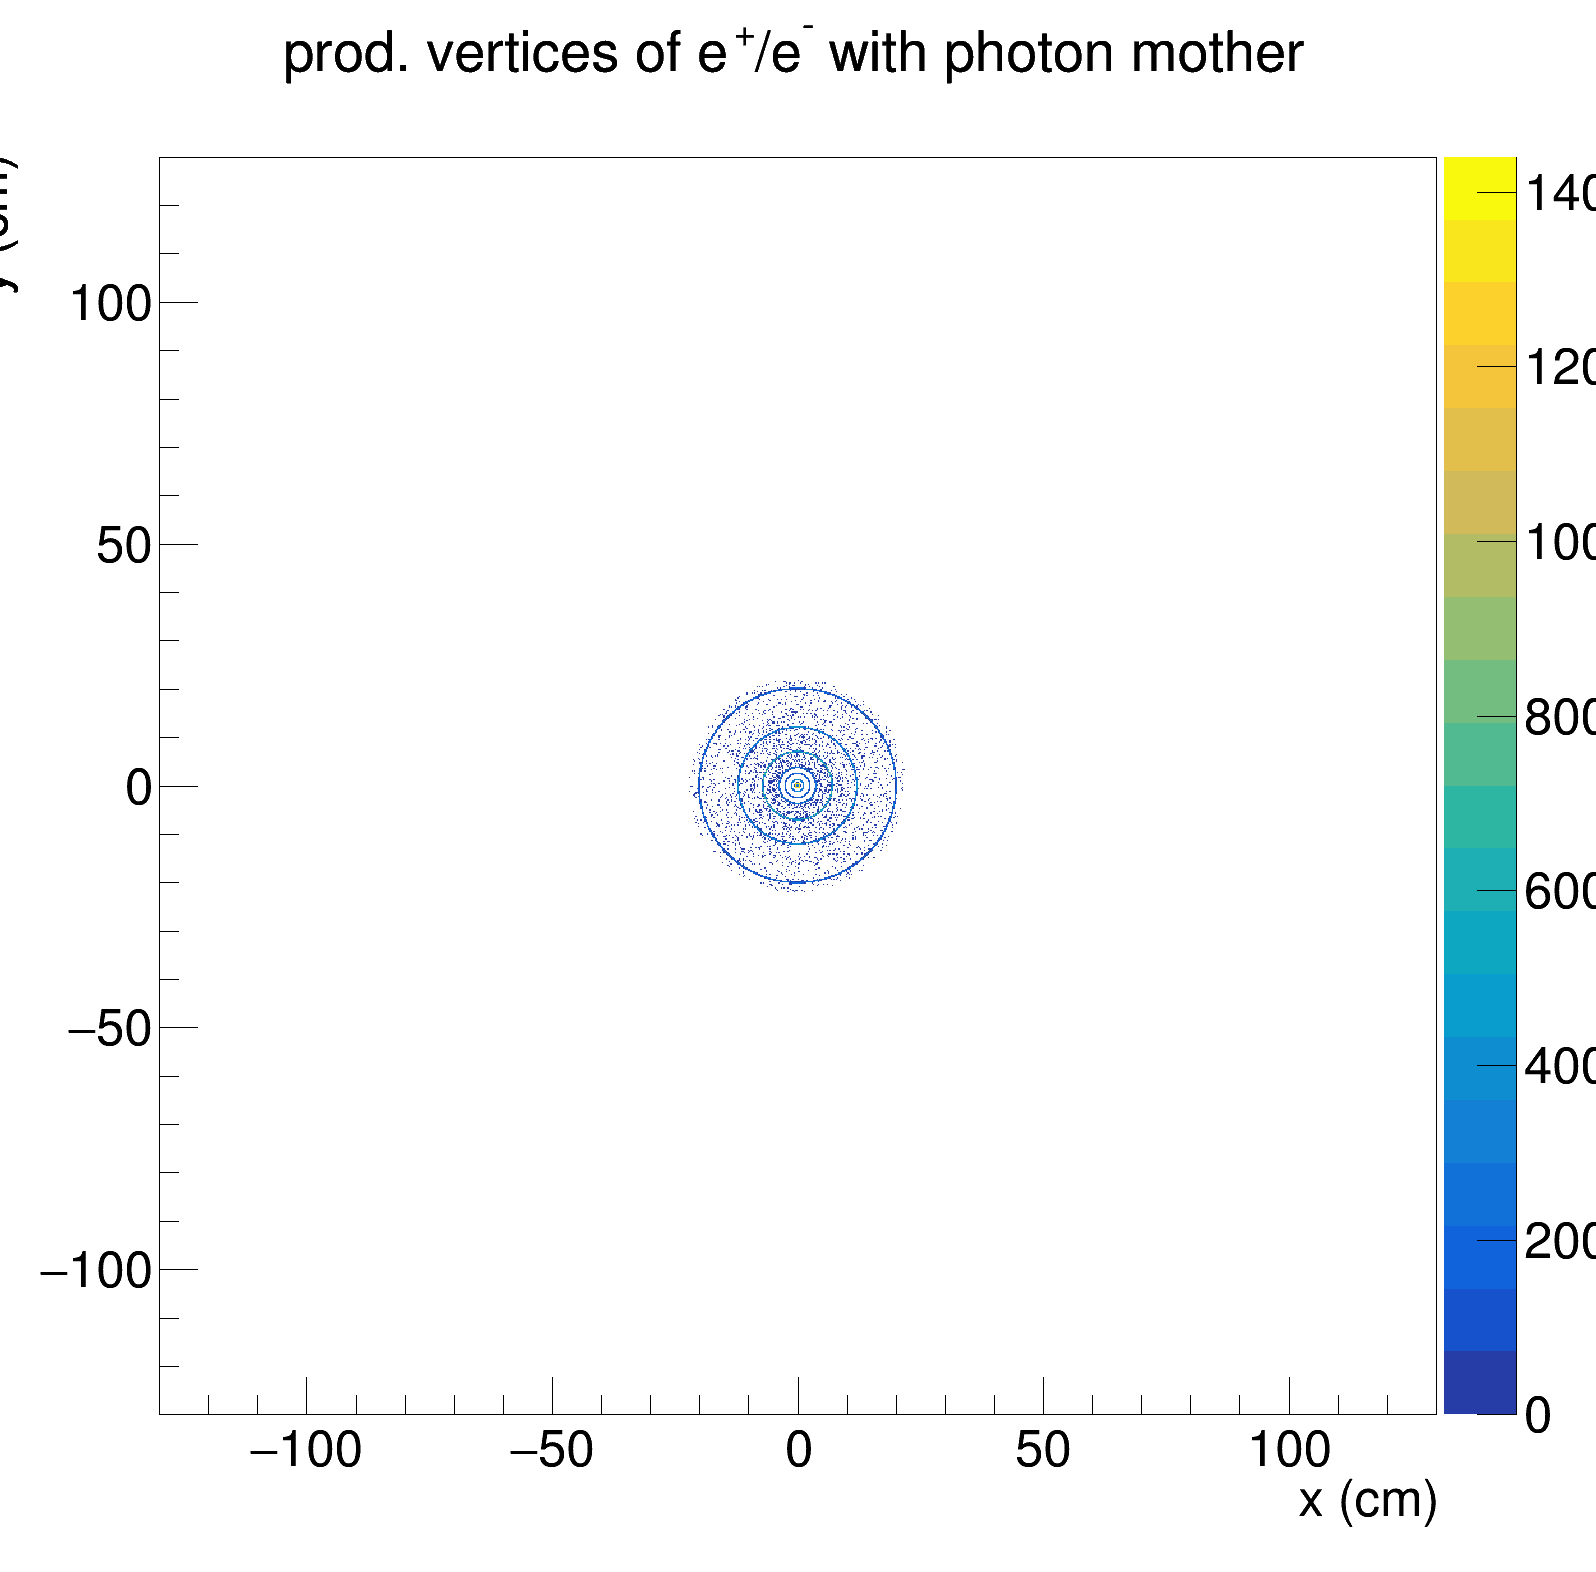
\includegraphics[width=0.28\textwidth]{/Users/marin/alice3/alice3Conversions//anaConv/saveAllR/conv_xy.png}\\
\end{tabular}

Tracker: 12 layers clearly visible\\
MC information used to located conversion vertices. \\
No reconstruction yet.

\end{frame}


\begin{frame}
\frametitle{Photon conversions}

Limit the conversion radius to 22 cm:\\
 7 layers for conversion and 5 layers for reconstruction\\

\begin{tabular}{cc}
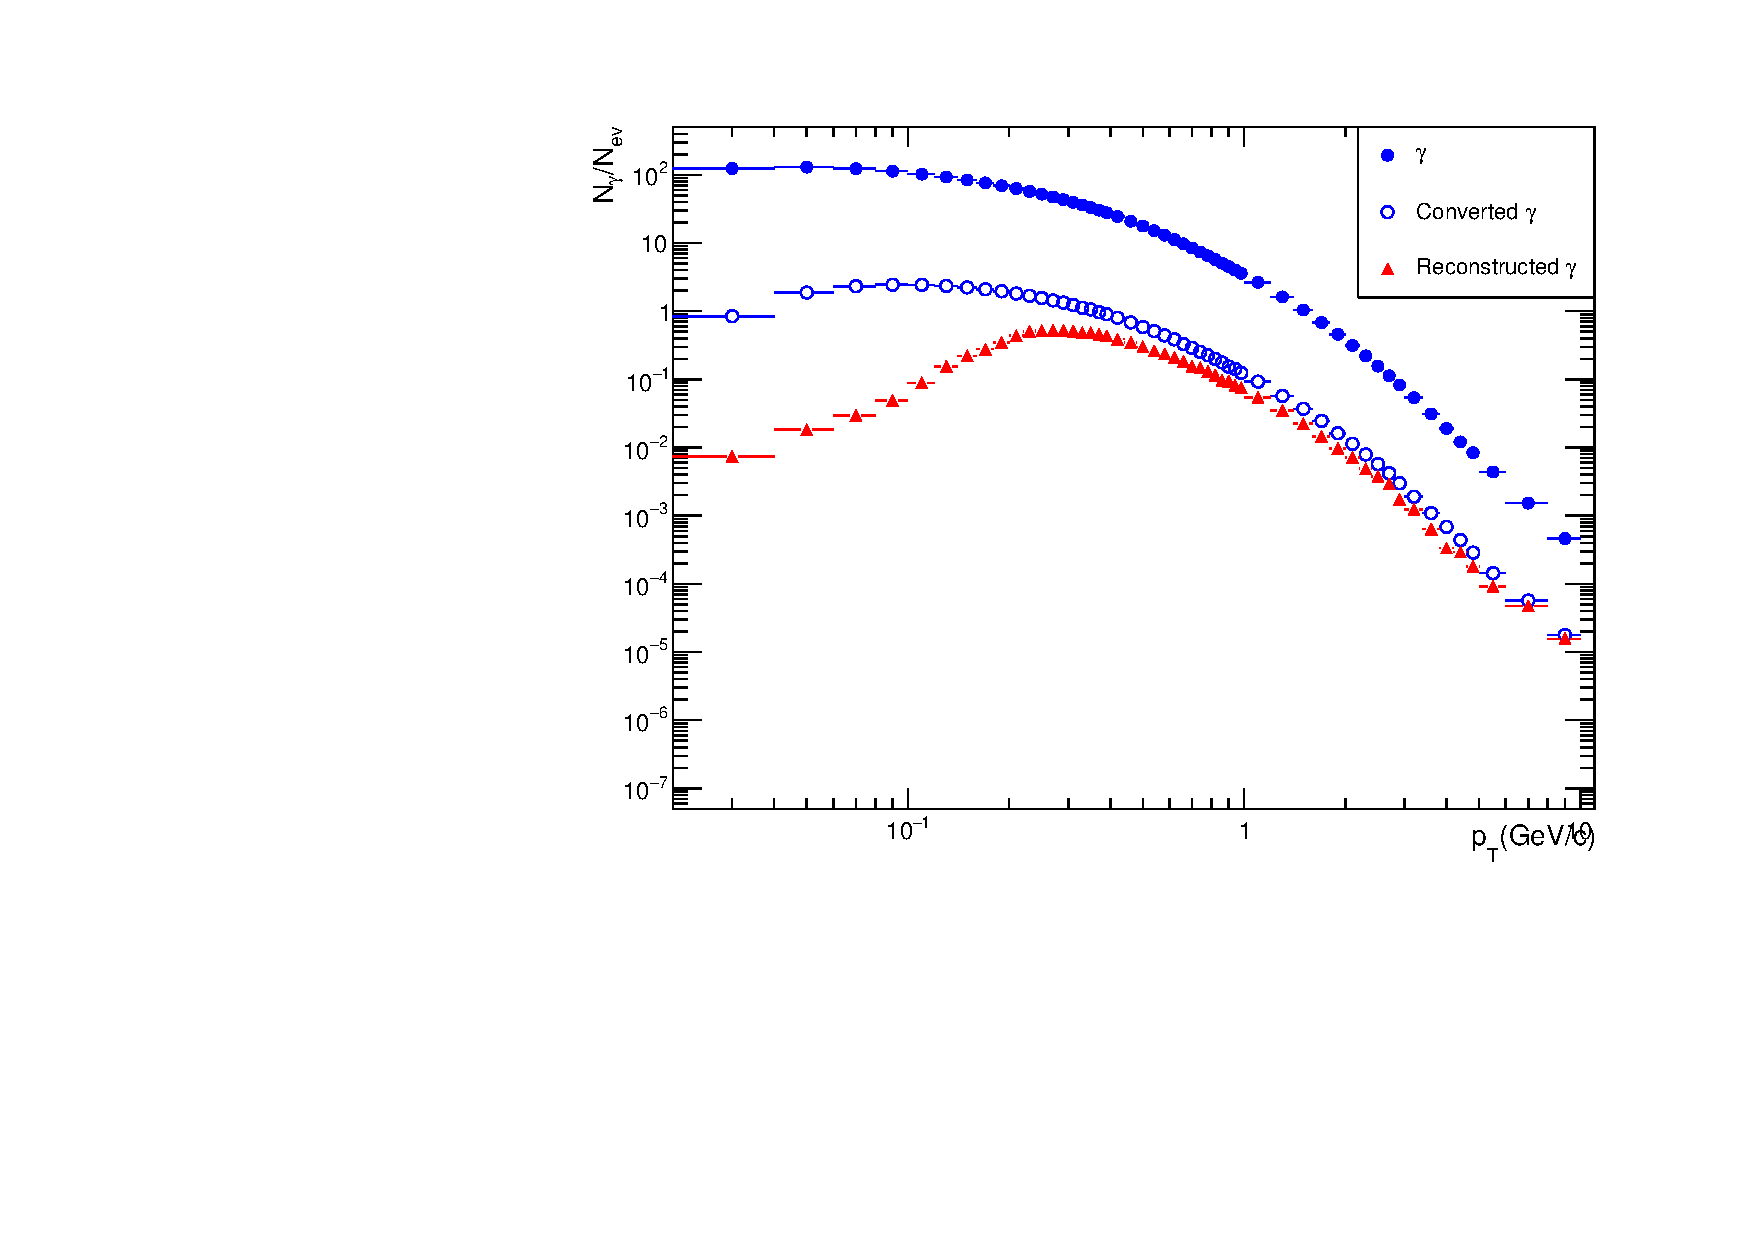
\includegraphics[width=0.33\textwidth]{/Users/marin/alice3/alice3Conversions//anaConv/PhotonPrimConvRec.pdf}&
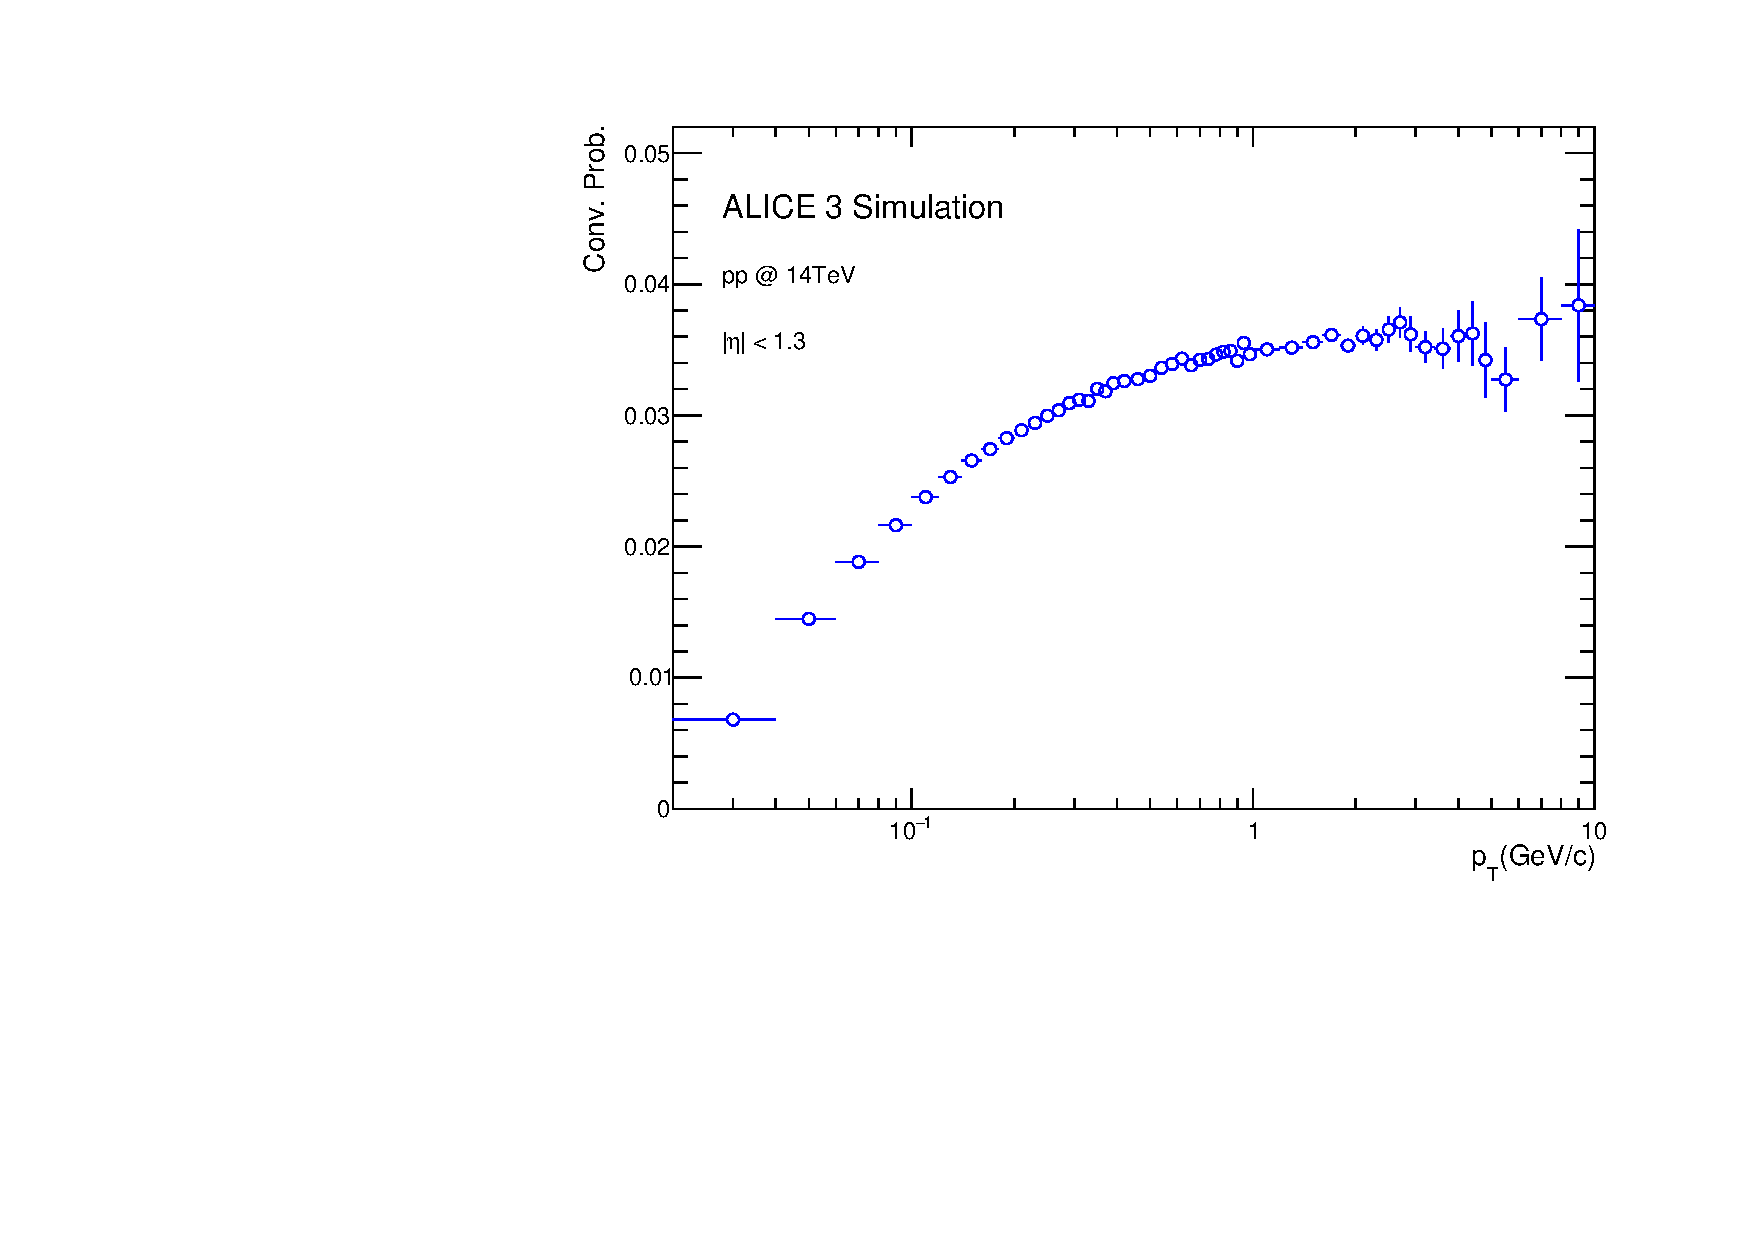
\includegraphics[width=0.33\textwidth]{/Users/marin/alice3/alice3Conversions//anaConv/PhotonConvProb.pdf}\\
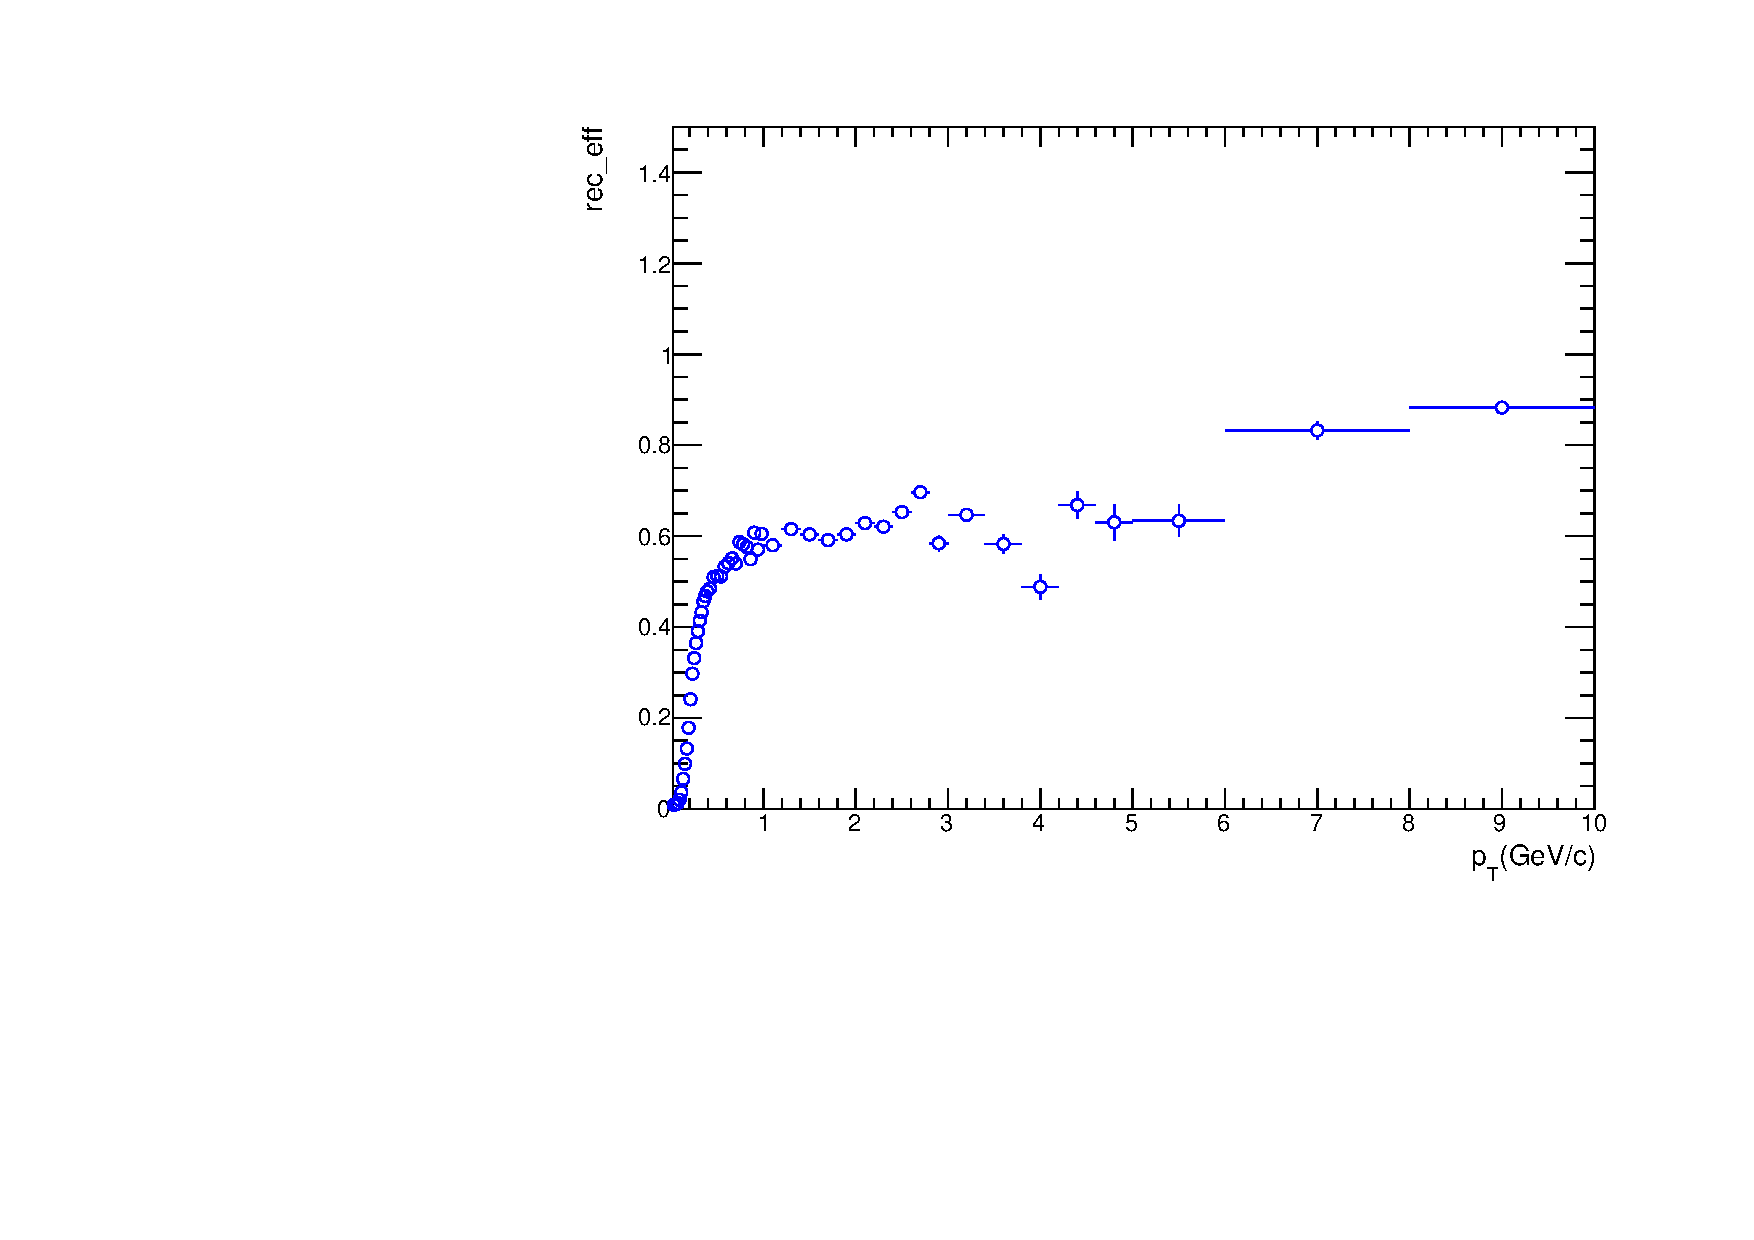
\includegraphics[width=0.33\textwidth]{/Users/marin/alice3/alice3Conversions//anaConv/PhotonRecEff.pdf}&
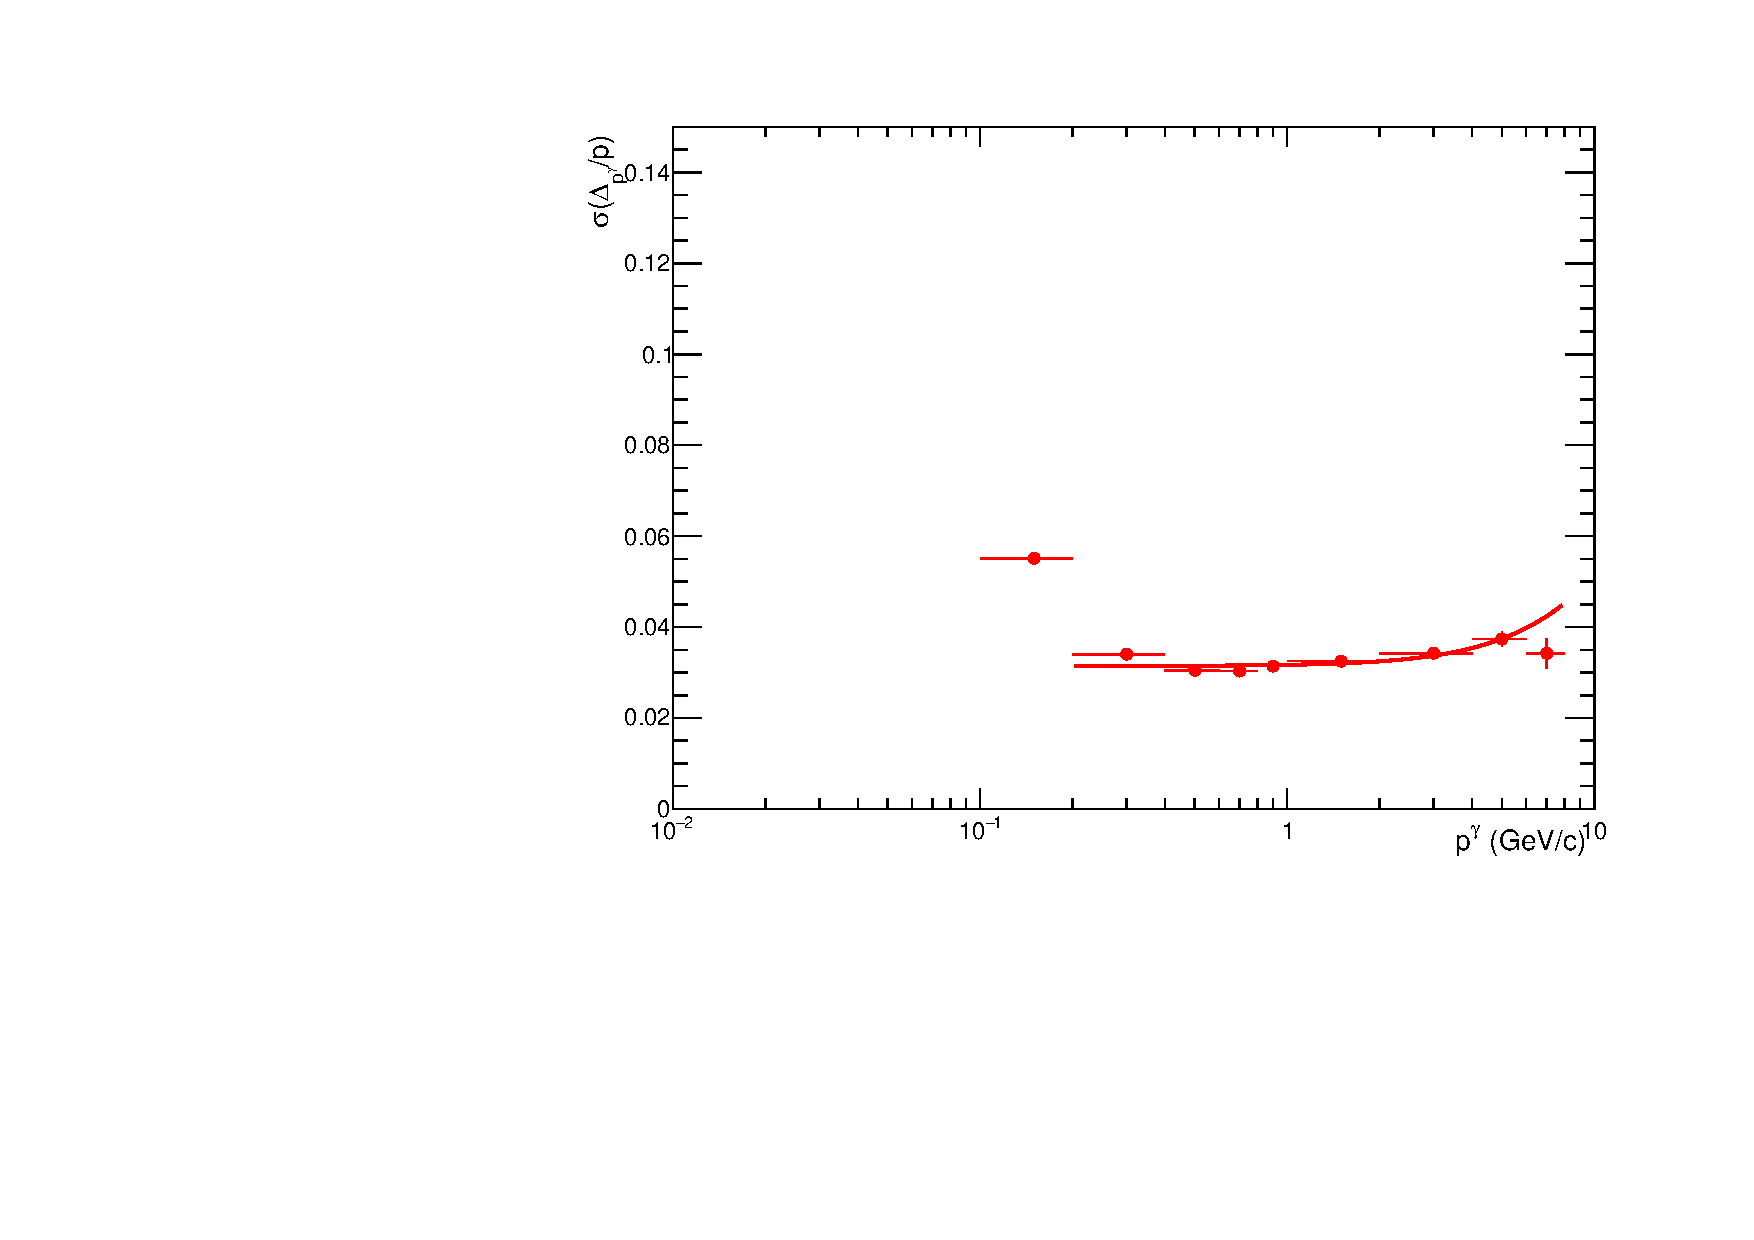
\includegraphics[width=0.33\textwidth]{/Users/marin/alice3/alice3Conversions//anaConv/PhotonResSigma.pdf}\\
\end{tabular}
\end{frame}

\begin{frame}
\frametitle{Photon conversions}
\begin{enumerate}
\item $\chi_C \rightarrow$ J/$\psi$+$\gamma$ simulation started using DelphesO2
\item $\gamma$ information and Preshower information stored in the AO2D.root
%\item Still need to lear how to analyse it
\end{enumerate}
\end{frame}




\begin{frame}
\frametitle{$\chi_C$}

\begin{tabular}{cc}
\includegraphics[width=0.4\textwidth]{/Users/marin/alice3/chic/ChicMassPCM.pdf}&
\includegraphics[width=0.4\textwidth]{/Users/marin/alice3/chic/chic_pT-pcm-recMatched.pdf}
\end{tabular}

\end{frame}



\end{document}




\begin{frame}
\frametitle{Photon conversions}

Limit the conversion radius to 15 cm: 6 layers for conversion and 6 layers for reconstruction

\begin{tabular}{cc}
\includegraphics[width=0.28\textwidth]{/Users/marin/alice3/alice3Conversions//anaConv/saveRMax15/conv_rz.png}&
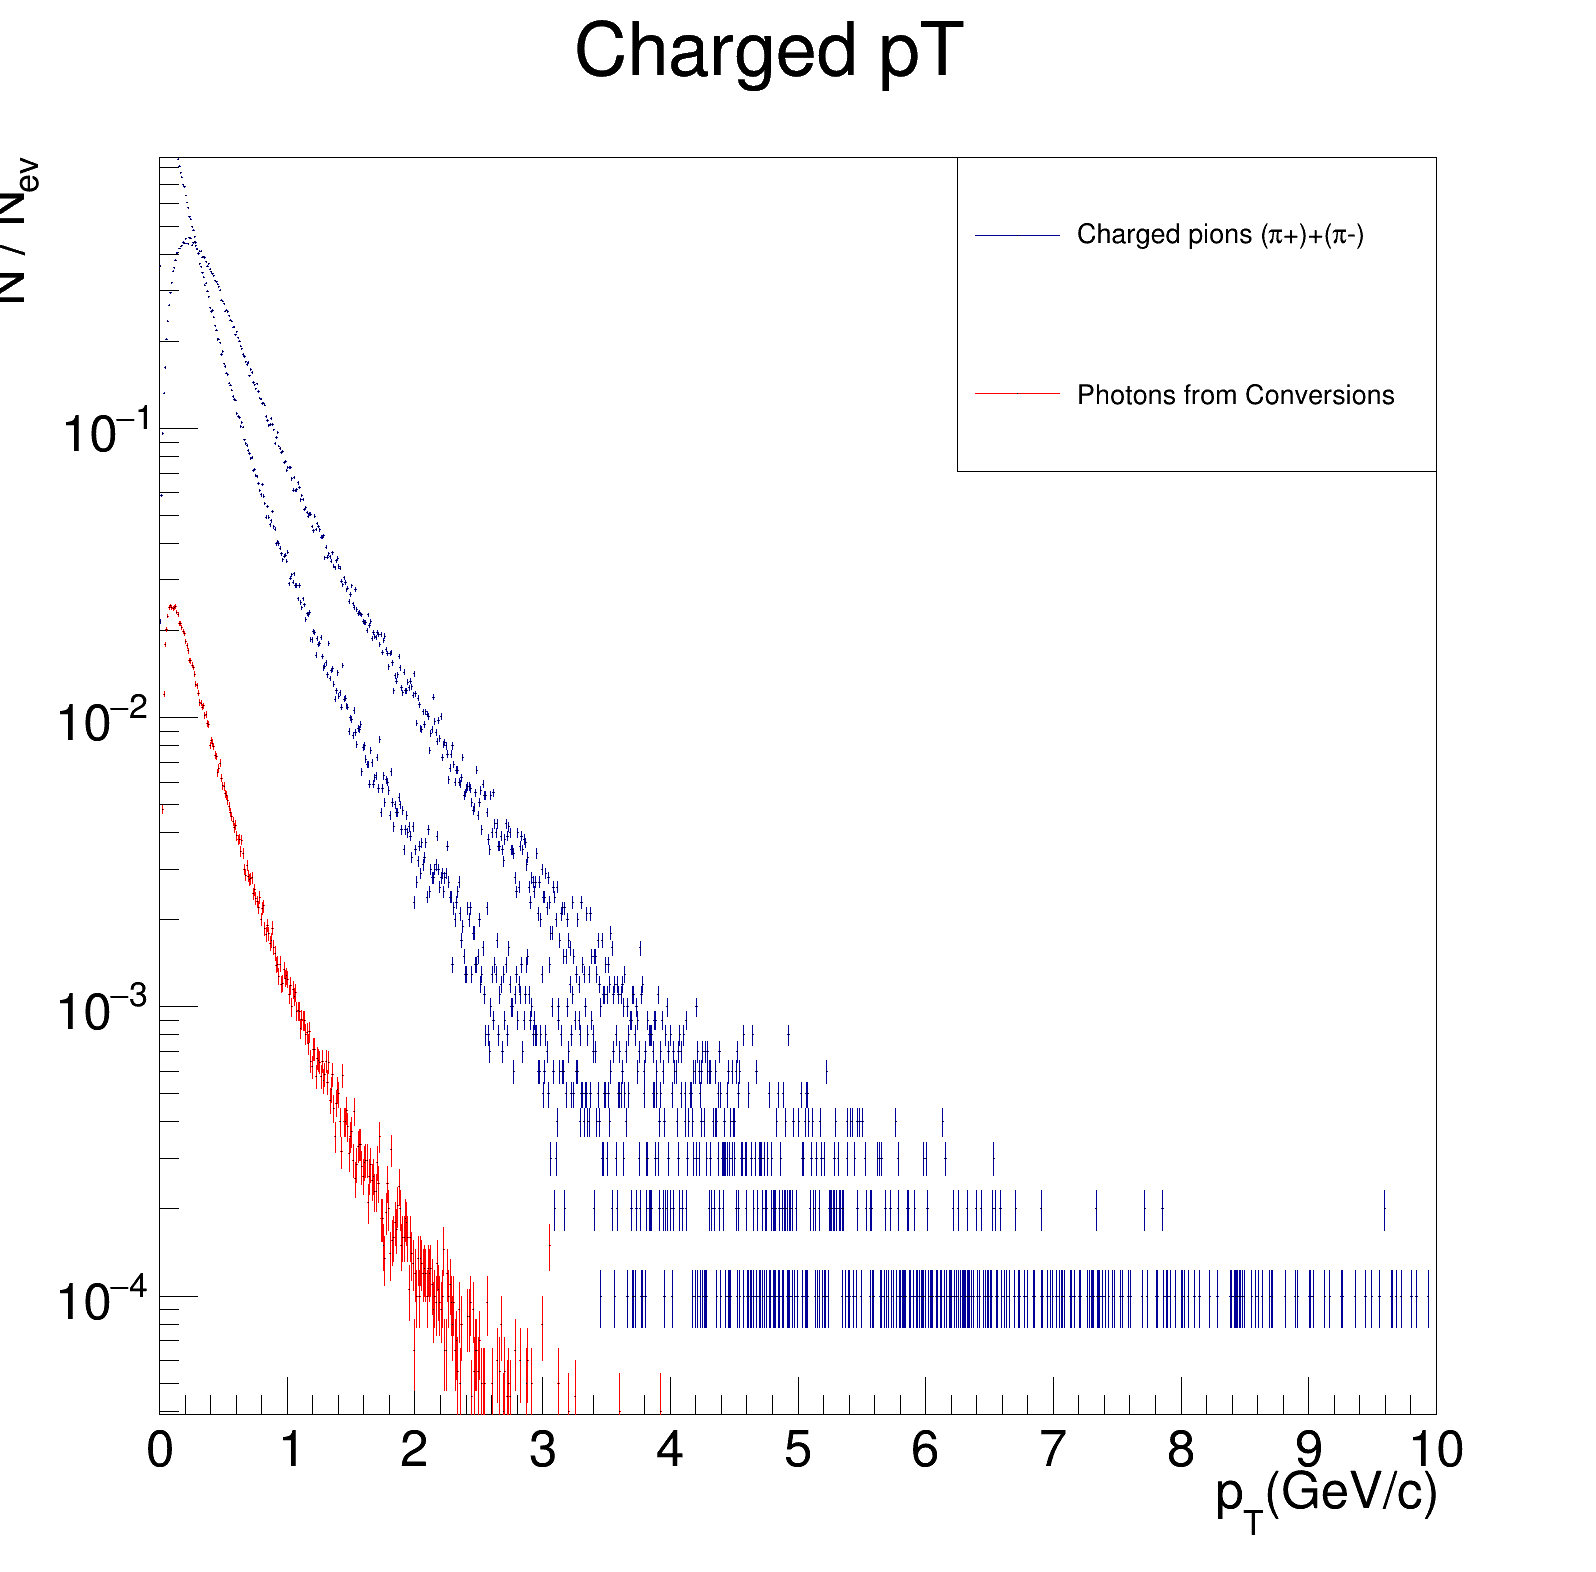
\includegraphics[width=0.28\textwidth]{/Users/marin/alice3/alice3Conversions//anaConv/saveRMax15/photon_pt.png}\\
\end{tabular}

MC info to obtain $\gamma$ \pT  \\

\begin{tabular}{cc}
events & 2.2  $ \cdot 10^6$  \\
$\gamma$ &  1.3 $ \cdot 10^6$   \\
$\pi^+$  & 2.47$ \cdot 10^7$  \\
$\pi^-$  & 2.47$ \cdot 10^7$  \\
\end{tabular}
% totGammaConv,totPiM, totPiP::495050  295787  5.57989e+06 5.57989e+06
\end{frame}





\end{document}
